% !TEX root = paper.tex
\section{Evaluation}

\name is evaluated on a commodity shared-memroy machine with two 14-core
Intel Xeon CPU E5-2697 v3 processors (28 cores total) running at 2.60GHz
(turbo-boost disabled) with 756GB of memory. The operating system is 64-bit
Ubuntu 16.04.5 LTS with GCC 5.5 (version 5.5.0 20171010) and LLVM Compiler
Infrastructure (version 5.0.2).


\name is evaluated against 12 C and C++ benchmarks, covering all the
DOALLable (showing speedup instead of slowdown) benchmarks from two
state-of-the-art automatic DOALL parallelization
papers~\cite{johnson:12:pldi,kim:12:cgo}. We also include one more
benchmark (179.art) from HELIX~\cite{simone:12:cgo}.

This work is focusing on boosting the efficiency of automatic
parallelization rather than increasing the applicability of it. This is
why we choose benchmarks that have been parallelized in prior work to
make a fair comparison.

These benchmarks are from five benchmark suites
(Trimaran\cite{trimaran:web}, SPEC\cite{}, PARSEC\cite{bienia:08:parsec},
MiBench\cite{guthaus:2001:iiwsc}). All PolyBench benchmarks and
\texttt{dijkstra} from MiBench are modified to accept command line
arguments and allocate arrays dynamically in the same way as
\cite{kim:12:cgo}. This modification is used to create bigger inputs, which
is necessary for separating profiling and evaluation input sets.

%
Each benchmark is profiled using a profiling input and all the following
experiments are conducted using a different, larger testing input.

\begin{table*}[h]
  % !TEX root = ../paper.tex
\small
\centering
\begin{tabular}{|l|c|c|l|l|}
\hline
Benchmarks & DOALL Coverage & Sequential Time & Arguments & Input    \\
\hline
doitgen    & 99.6\%  & 1034.86 & 768 768 768 & -  \\
\hline
enc-md5    & 100.0\% & 174.26    & 1000 & -  \\
\hline
covariance & 99.9\%  &     & 4096 4096 & -  \\
\hline
swaptions  & 100.0\% & 1546.29   & -ns 10000 -sm 40000 -nt 1 & -  \\
\hline
3mm  & 100.0\%       & 3515.78   & 4096 4096 4096 4096 4096                & -  \\
\hline
gemm       & 100.0\% & 1182.50   & 4096 4096 4096                    & -  \\
\hline
179.art    & 99.1\%  & 702.32    &
{\parbox[l]{5cm}{-scanfile c756hel.in \\-trainfile1 a10.img \\-trainfile2 hc.img\\ -stride 1 -startx 60 \\-starty 90 -endx 210 \\ -endy 240 -objects 10}} & input1   \\
\hline
dijkstra-dynsize & 99.7\%  &     & ../input3000/input3000.in 3000                & input300 \\
\hline
blackscholes & 99.7\% & 4702.20   & 1 in\_10M.txt out\_10M.txt                & ref      \\
\hline
2mm  & 100.0\%       & 2360.60   & 4096 4096 4096 4096               & -  \\
\hline
052.alvinn & 97.5\%  &     & 60000                 & input 1  \\
\hline
correlation & 99.7\%  & 914.39    & 4096 4096                   & - \\
\hline
\end{tabular}
  \caption{
    Benchmark Details: (a) Execution time coverage is the percentage of
  execution time of paralleized loops. Based on it, the theoretical max
  speedup is calculated using Amdahl's Law with the assumptions of no
  overheads and 28 workers. \\(b) SAMA's (Speculation-Aware Memory
  Analyzer's) coverage is the number and percentage of dependences handled
  by SAMA that were unresolved by static analysis alone. Entries denotes by
  ``N/A'' indicate all dependences are handled by static analysis. \\(c)
  Proposed enablers’ coverage is the number and percentage of objects
  covered by efficient speculation privatization transformations proposed
  in this work. (d) Private read and write sizes are measured using the
  test input for each benchmark. \namensp\textsubscript{v1} stands for
  \name with only planner; \namensp\textsubscript{v2} stands for \name with
  planner and propsed enablers.}
  \label{tab:benchmark-list}
    \vspace{-5pt}
\end{table*}

\subsection{Parallelization Performance}

\begin{figure*}[ht]
  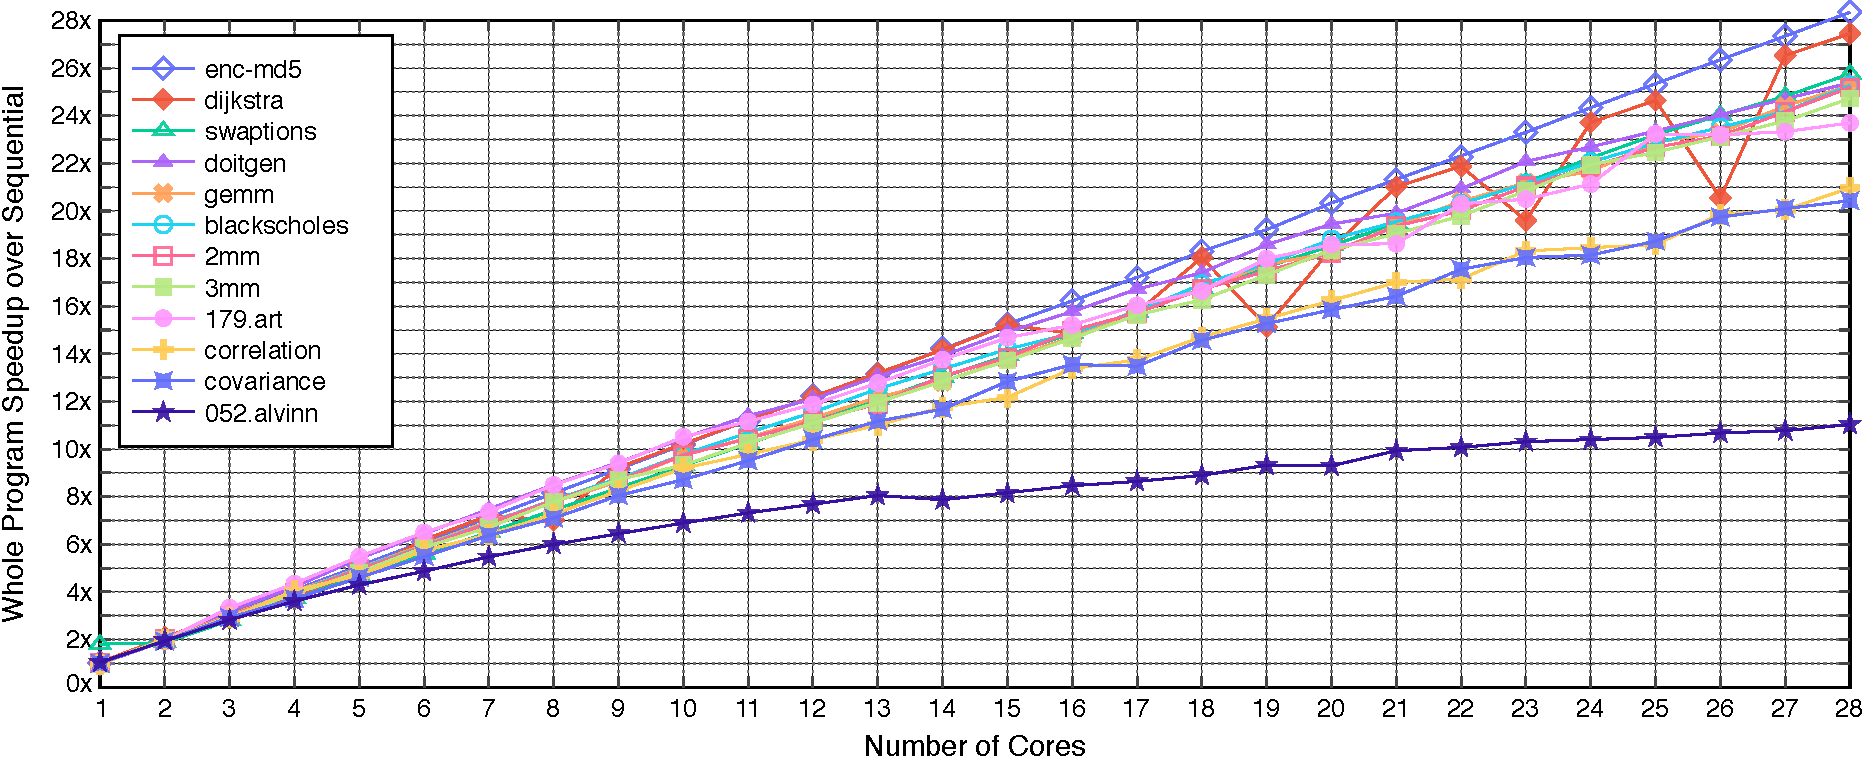
\includegraphics[width=\textwidth]{figures/multi-core-crop}
  \caption{Fully Automatic Whole Program Speedup over Best Sequential}
  \label{fig:multi-core-scale}
\end{figure*}

Figure \ref{fig:multi-core-scale} presents whole program speedups for
all benchmarks running with different numbers of cores. These speedups are
relatvie to the best sequential performance of the original code, compiled
with \texttt{clang++ -O3}. \name achieves scalable performance on all the
benchmarks.

% enc-md5, swaptions, gemm, 3mm, 2mm, blackscholes, doitgen
\texttt{enc-md5}, \texttt{swaptions}, \texttt{gemm}, \texttt{2mm},
\texttt{3mm}, \texttt{blackscholes}, and \texttt{doitgen} show a
scalability close to linear. This performance comes from most memory
objects being privatized with little or no overheads.

% dijkstra
The \texttt{dijkstra}, having a lot of memory operations like
\texttt{malloc} inside the inner loops, manifests a significant variance in
the runtime.

% 052.alvinn
\texttt{052.alvinn} exhibits a lower speedup (11$\times$ on 28
cores) than other benchmarks. This results from the parallelizable loop
being a nested inner loop with 97.5\% execution time coverage of the whole
program with the testing input, which results in 16.7$\times$
theoretical maximum speedup based on Almdahl's Law.
% 179.art
\texttt{179.art} whose theoretical maximum speedup is 22.5$\times$, due to
the same effect, shows a smaller scaling factor close to the bound. Note
that HELIX\cite{simone:12:cgo} reports 4.2$\times$ speedup on 6 cores while
\name exhibits 6.5$\times$, showing that an efficient speculative approach
can even overcome a static approach in terms of speedup.

% correlation and covariance
\texttt{correlation} and \texttt{covariance} have complicated triangle(?) WAW
dependence patterns which cannot be resolved by static analysis or cheap
privatization variants. As a result, the corresponding memory objects are
classified as private and need logging and merging for write sets,
resulting in lower speedups.

\begin{figure*}[ht]
  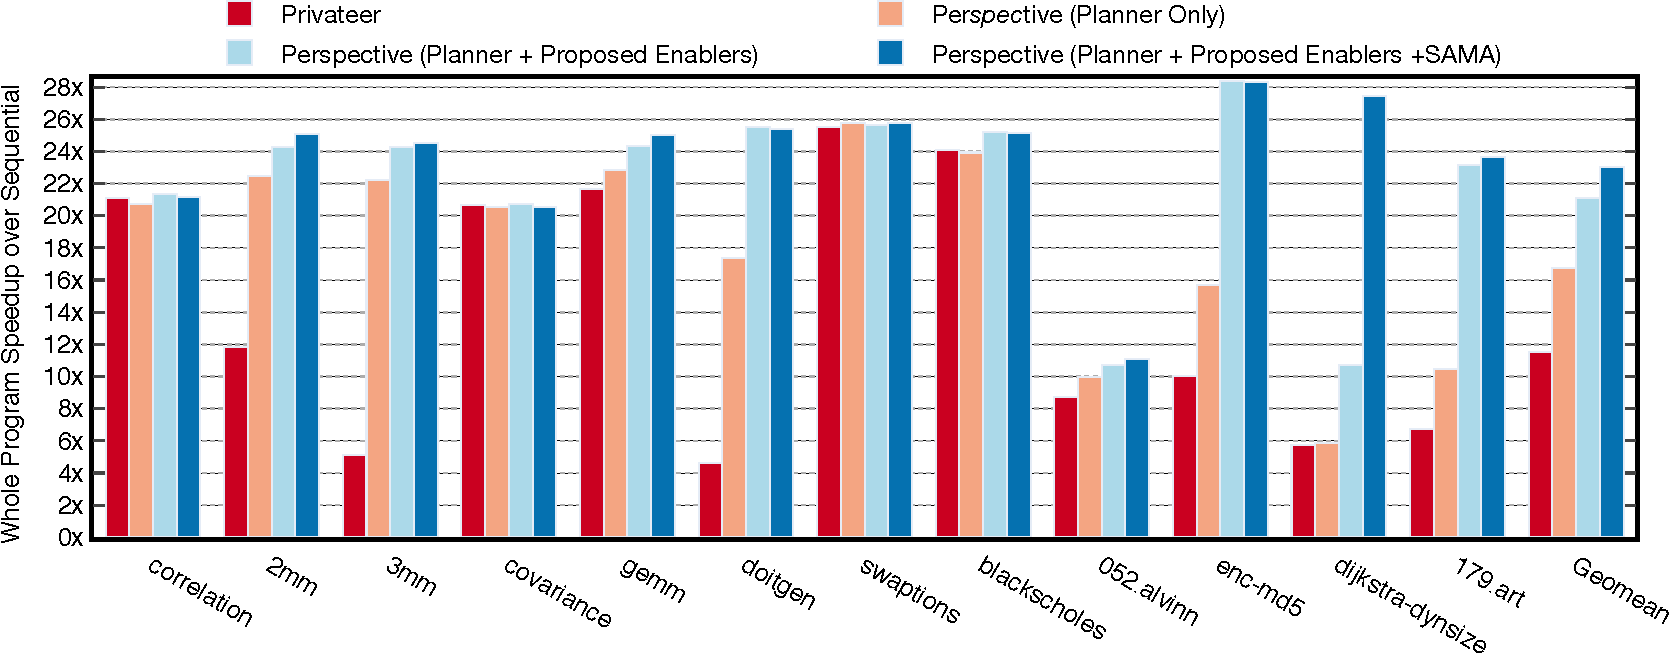
\includegraphics[width=\textwidth]{figures/compare-privateer}
  \caption{Whole Program Speedup Comparison among variants of \name and Privateer with 28 Cores}
  \label{fig:speedup-compare}
\end{figure*}

Figure \ref{fig:speedup-compare} compares \namensp's resultsw
 with two
variants of Privateer and one variant of \namensp. The first bar shows the
performance of Privateer implemented with the best practice assumption(?).
Some peephole optimizations are used to reduce the use of memory
speculation and to hoist memory check out of the inner loops. The speedup
and runtime breakdown results match the description in the paper. Although
being the state-of-the-art framework in terms of applicability, Privateer
missed some opportunities to remove some read checks as mentioned in
STMLite\cite{mehrara:09:stmlite} and ClusterDOALL\cite{kim:12:cgo}. To
improve as much as possible on top of Privateer, we utilize static analysis
including a stronger KillFlow analysis pass to remove read checks.
\texttt{2mm}, \texttt{3mm}, \texttt{doitgen}, \texttt{enc-md5}, and
\texttt{179.art} benefit from this improvement as shown in the second bar.
Note that \textbf{ref XXX} if all dependences are removed statically, no
checkpoint is needed in the runtime.

The third bar presents the results of a variant of \name without the cheap
privatization transformations proposed in \ref{}. Parallelization through
\name, which incorporates speculation-aware-memory-analysis and cheap
privatization transformations, is presented in the fourth bar, achieving
23.0$\times$ speedup compared to 11.5$\times$ by the original Privateer.


% \subsubsection{Effect of parallelization on vectorization}

% instrumentation kills vectorization


% \subsection{Static Analysis and Enablers}
% Figures Needed:
% \begin{itemize}
% % (no need, just discuss the use of CAF in previous sections) \item CAF:
% % with and without; no topping; with only BasicLoopAA and ScevAA

% % (no need, show in the benchmark table) \item Coverage: Spec-DOALL
% % percentage of coverage of each benchmark
% \item Enablers: Enablers used for each benchmark
% \item Optimization level: Performance with different optimization levels
% \end{itemize}

% Discussion Needed:

% Present in a table, which enablers were used for all benchmarks

\subsection{Overhead Breakdown}

% \begin{figure*}[htp]
%   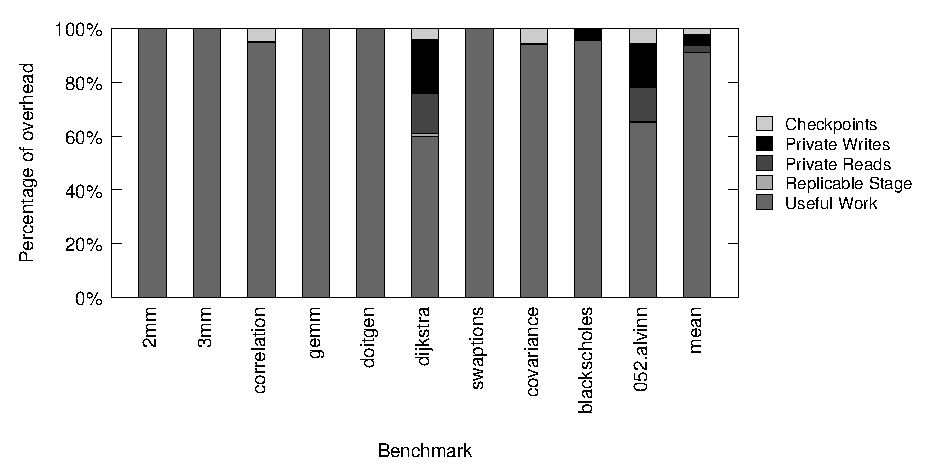
\includegraphics[width=0.9\textwidth]{figures/overheads}
%   \label{fig:overheads}
%   \caption{Overhead comparison with various enablers disabled}
% \end{figure*}
% \begin{figure*}[htp]
%   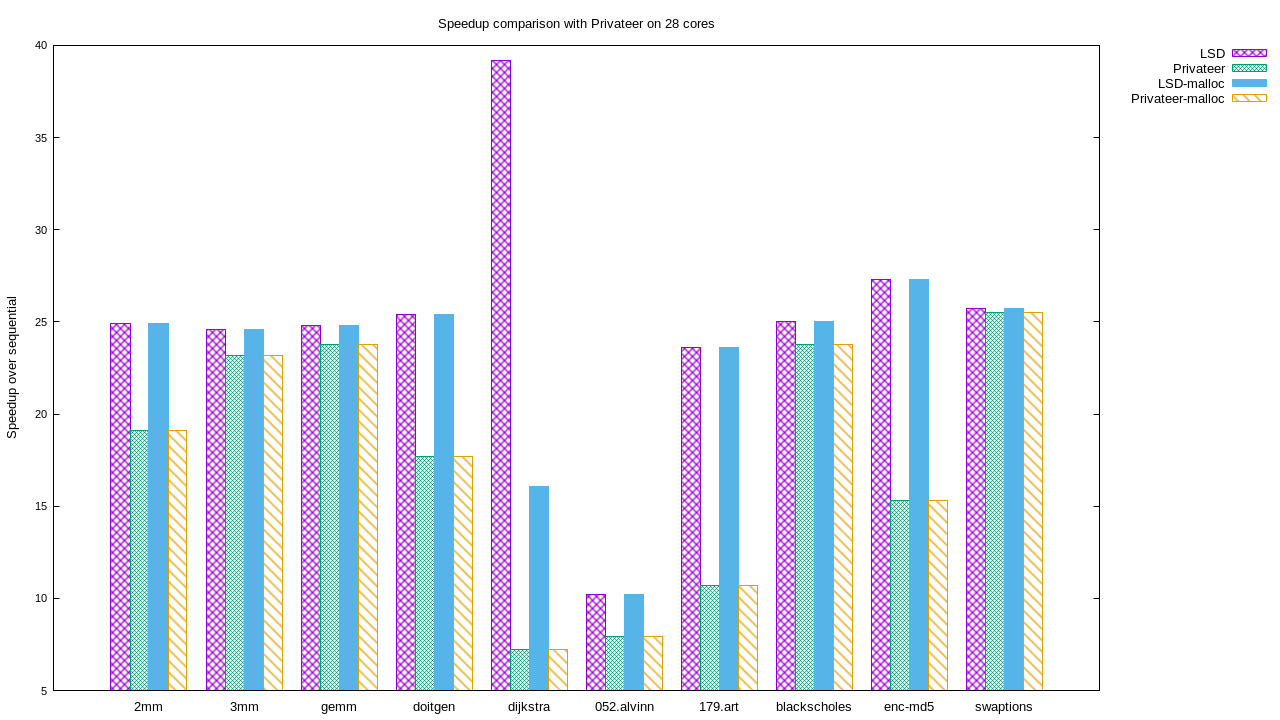
\includegraphics[width=0.9\textwidth]{figures/comparison}
% \end{figure*}
% Huge speedup for dijkstra is largely due to the cheaper "malloc" that
% we use in our heaps. Using a similar malloc in the sequential version
% yields ~16x speedup in dijkstra and insignificant difference in the
% other benchmarks.
% Shown in Figure \ref{fig:overheads} is the overhead breakdown of each
% benchmark comparing \name with various enablers disabled. The useful work
% of \name is normalized to 100\%, with the others being scaled accordingly.
% These result demonstrate the correlation between the sum of the overheads
% to the speedup that can be achieved. \{\textbf{XXX} Something about
% how we remove dependences with redundant private read elimination,
% the new kill\_private heap, and collaboration \}
Table \ref{tab:benchmark-list} shows the overhead of private reads and
writes for each of the variants of Privateer and \namensp. These results
demonstrate the correlation between the overheads and the speedup that can
be achieved. Redundant read elimination \{\textbf{XXX is this the right
name?}\} removes reads that can be statically be inferred to never fail.
Using cheap speculation, we are able to move some of the private objects to
the heaps that do not require expensive logging and checks.
Using collaboration removes the remaining unnecessary logs that cannot
be removed with static analysis alone.

For most of the benchmarks, checkpointing does not add any
significant (over 1\%) overhead; the exceptions are
\texttt{052.alvinn}, \texttt{correlation}, and \texttt{covariance}.
The inner loop of \texttt{052.alvinn} is chosen for parallelization --
because the useful work of the loop is small and runs for 60,000
iterations, checkpointing constitutes a considerable portion of the run
time, \textasciitilde20\%. For \texttt{covariance} and \texttt{correlation},
the speculation-aware memory analyzer could not avoid using memory
speculation and as such, the checkpoints need to merge large private sets
with an overhead of \textasciitilde10\% for both.

\subsection{Misspeculation Analysis}
\begin{figure}[htp]
  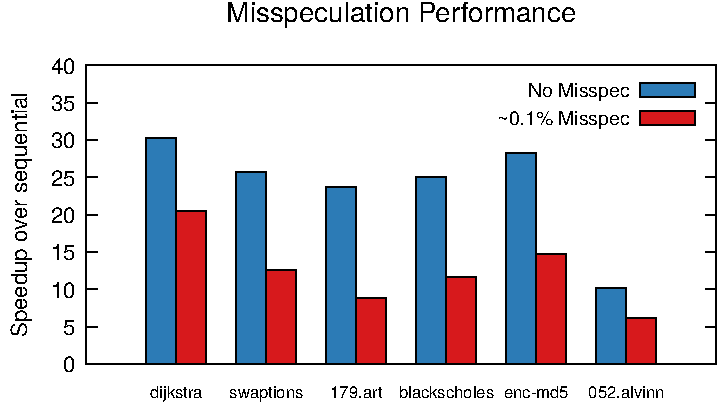
\includegraphics[width=\columnwidth]{figures/misspec-crop}
  \caption{Misspeculation performance across speculative benchmarks}
  \label{fig:misspec}
\end{figure}
Figure \ref{fig:misspec} shows how misspeculation affects the
performance of the six speculative benchmarks with a misspeculation rate of
0.1\%. Since none of the benchmarks exhibit misspeculation on the
given input sets, we artificially inject misspeculation at the end of
every 1000 iterations to observe the performance degradation.
Note that for many benchmarks, speculation is only used
because analysis cannot disprove a dependence, even though manually
examining the source code reveals that the dependence will never manifest.
Thus, the only place misspeculation can possibly occur is during a heap
check.
% Note that misspeculation with \name is extremely unlikely, as
% static analysis can disprove many speculative assumptions and for many of
% the benchmarks, misspeculation is only possible during a heap check.
The inputs for \texttt{179.art} were not large enough to have
enough iterations for misspeculation at this rate, so we perform a
weighted average of non-misspeculating and misspeculating runs to achieve
an average corresponding to the respective rate.
These results demonstrate that \name performs well with only high
confidence speculation.
Systems that have larger overheads have a larger chance of speculation (since
they use more speculative assumptions), but we minimize the amount of speculation.
\{\textbf{XXX} Reword this\}
% As the iteration within a checkpoint that misspeculation
% occurs can affect the recovery cost, we inject these misspeculations in the
% middle of a checkpoint chunk (\textbf{XXX} find better wording) to have a more
% realistic simulation, assuming that programs can misspeculate at any iteration with a
% uniform distribution.

% \subsection{Power Consumption}

% Power and energy stats here

